\subsection{Разработка интерфейса взаимодействия}

Интерфейс взаимодействия с пользователем основан на HTML с применением
технологии Ajax с целью повысить удобство использования. Такой выбор был сделан на
основе специфики разрабатываемой системы и анализа требований к веб-приложению.
Необходимым условием взаимодействия пользователя с системой является наличие
современного веб-браузера, поддерживающего язык JavaScript и спецификацию HTML 4.0
(Mozilla Firefox 4.0, Google Chrome 10 и т.п.).

\subsubsection{Разработка графа диалога}

Граф диалога проектируемой подсистемы:

\begin{figure}[!h]
\centering
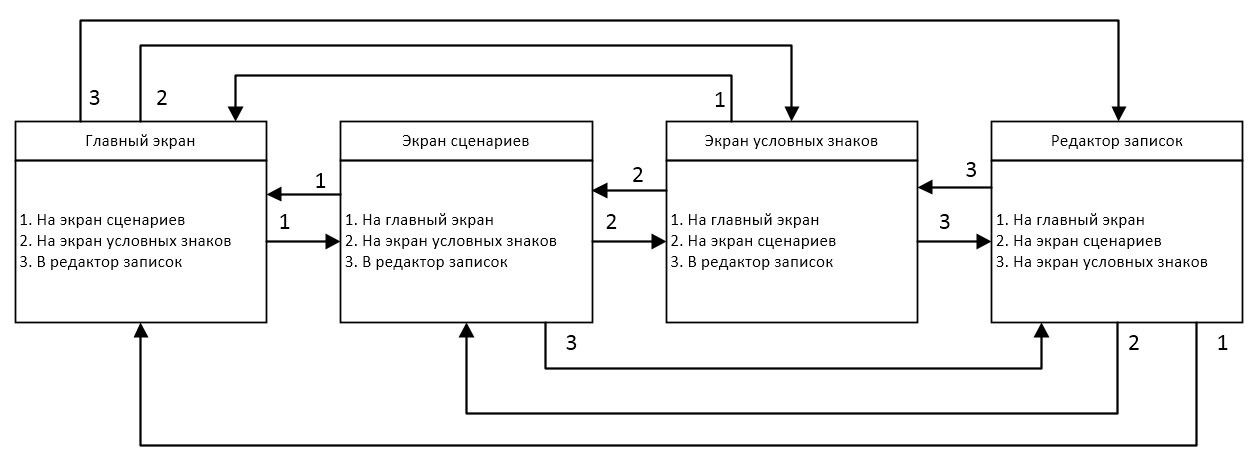
\includegraphics[width=\textwidth]{technology/graph}
\caption{Граф диалога.}
\label{figure:dialogGraph}
\end{figure}

\subsubsection{Разработка экранных форм}

Для разработки экранных форм выбрана библиотека Bootstrap, обеспечивающая эргономический и единообразный интерфейс, что соответствует требованиям проекта.

\subsection{Описание экранных форм}

\begin{figure}[!h]
\centering
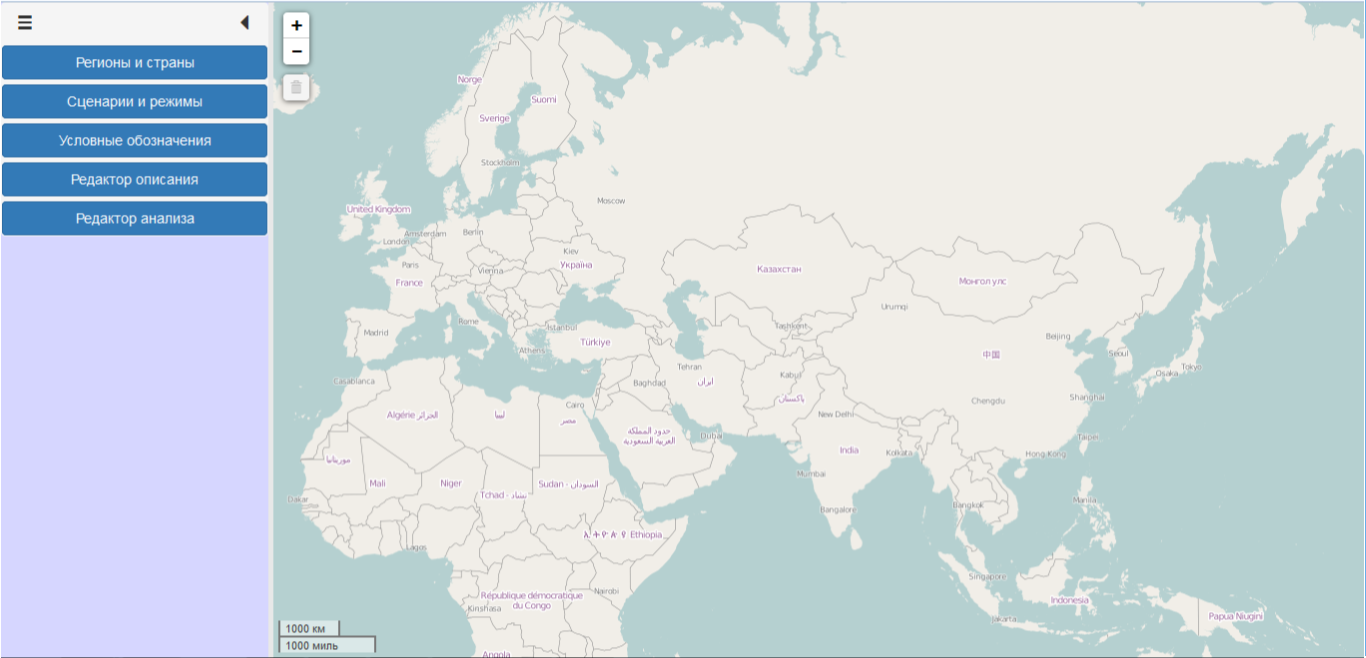
\includegraphics[width=\textwidth]{technology/gui/1}
\caption{Начальный экран.}
\label{figure:gui1}
\end{figure}

Слева представлено основное меню клиентского приложения. Карта продолжает отображаться при выборе любого из пунктов меню.

\clearpage
\begin{figure}[!h]
\centering
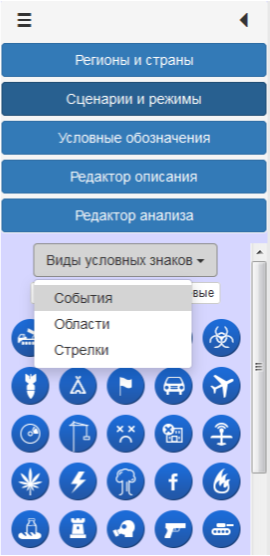
\includegraphics{technology/gui/2}
\caption{Виды условных знаков.}
\label{figure:gui2}
\end{figure}

Приложение поддерживает три типа условных знаков:

\begin{itemize}
\item События -- для отметки точечных событий, объектов
\item Области -- для отметки распределённых по площади объетов: позиций сторон, площадей затопления, возгорания итп.
\item Стрелки -- для отметки передвижения, направления распространения объектов 
\end{itemize}

\clearpage
\begin{figure}[!h]
\centering
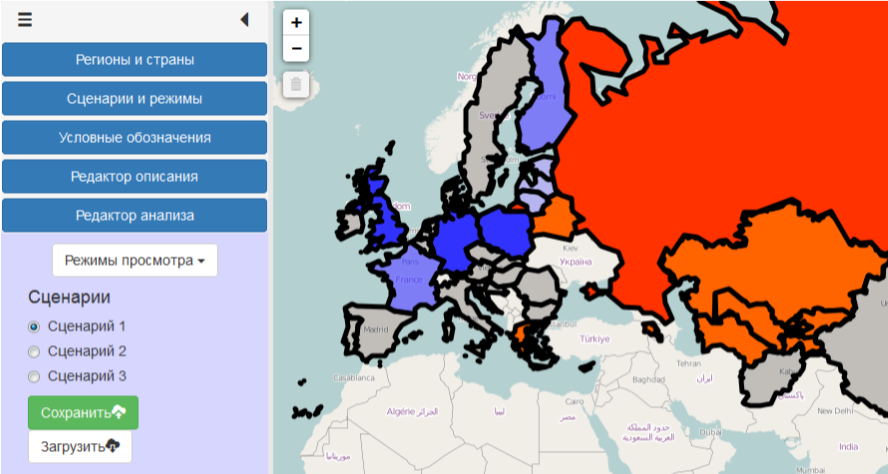
\includegraphics[width=\textwidth]{technology/gui/3}
\caption{Интенсивность новостей по странам.}
\label{figure:gui3}
\end{figure}

В этом режиме отображения с помощью тепловой карты отображается скорость поступления новостей по странам.

\begin{figure}[!h]
\centering
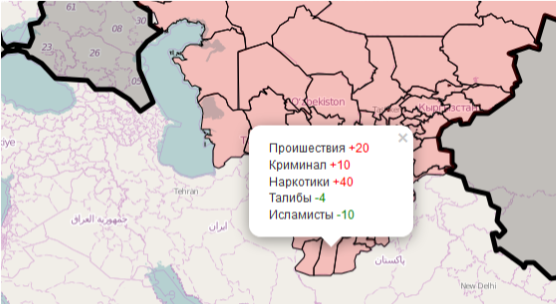
\includegraphics[width=\textwidth]{technology/gui/4}
\caption{Пример отображения прогноза.}
\label{figure:gui4}
\end{figure}

Пример отображения прогноза: при клике левой кнопкой мыши на провинцию, появляется всплывающее окно с пятью наиболее активными темами данной провинции и рядом с ними даётся прогноз изменения активности -- количества новостей за период времени, на прогнозируемый период.

\begin{figure}[!h]
\centering
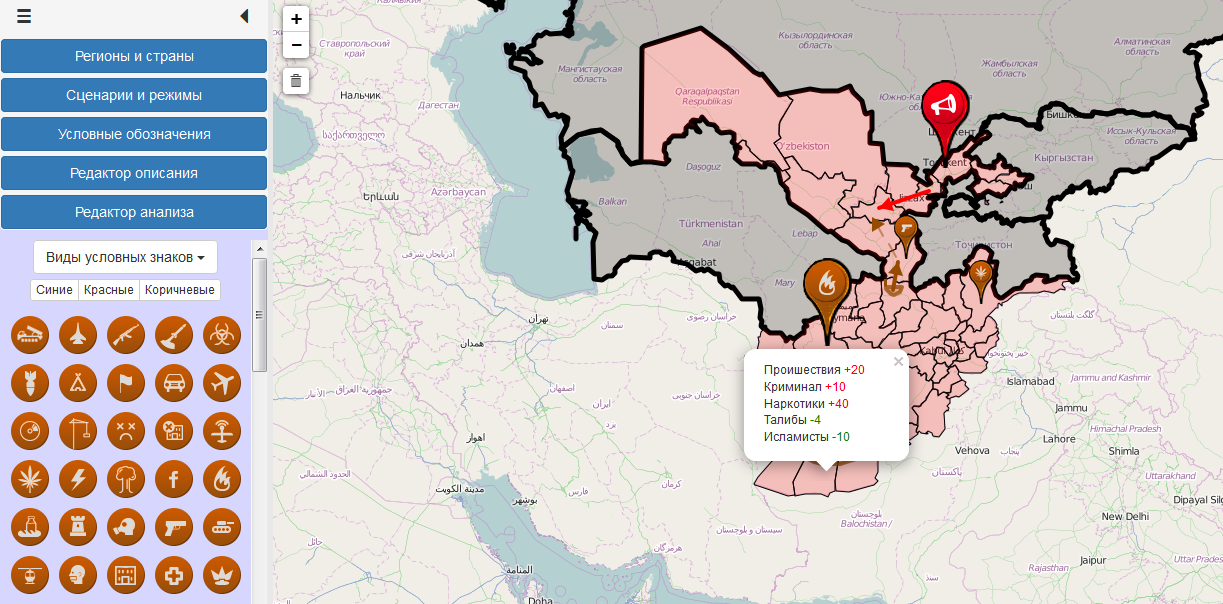
\includegraphics[width=\textwidth]{technology/gui/5}
\caption{Пример сценария.}
\label{figure:gui5}
\end{figure}

Сценарий по замыслу представляет собой набор элементов карты.

\begin{figure}[!h]
\centering
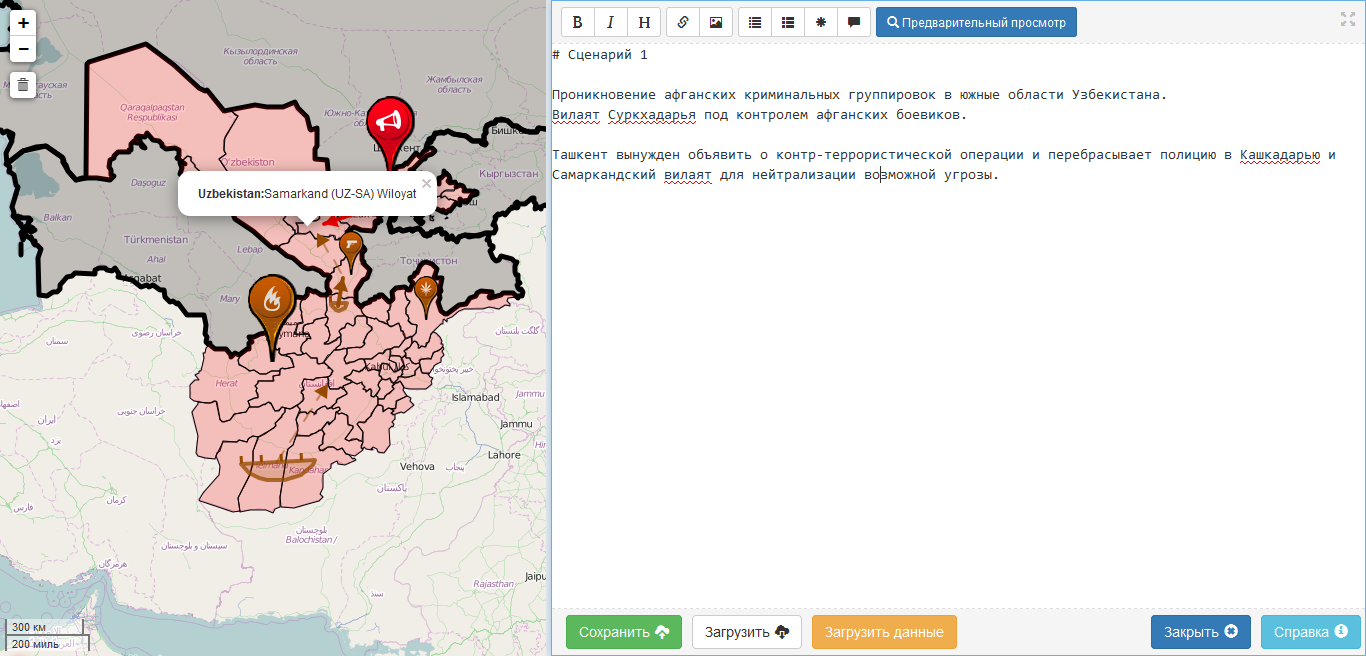
\includegraphics[width=\textwidth]{technology/gui/6}
\caption{Редактор аналитической записки.}
\label{figure:gui6}
\end{figure}

Аналитическая записка является сопровождением к сценарию и составляется в разметке markdown.